\title{
	
\includegraphics[scale=0.2,keepaspectratio]{eps5black}\\
	\sanskrit गीतोच्चारण}
\author{\sanskrit विश्वजीत अग्रवाल}
\date{January 2021}
\maketitle
\begin{quotation}
	\begin{center}\sanskrit
	यदा यदा हि धर्मस्य ग्लानिर्भवति भारत  । 
	
	अभ्युत्थानमधर्मस्य तदाऽऽत्मानं सृजाम्यहम्  ॥ 
\end{center}
\end{quotation}
\begin{center}
	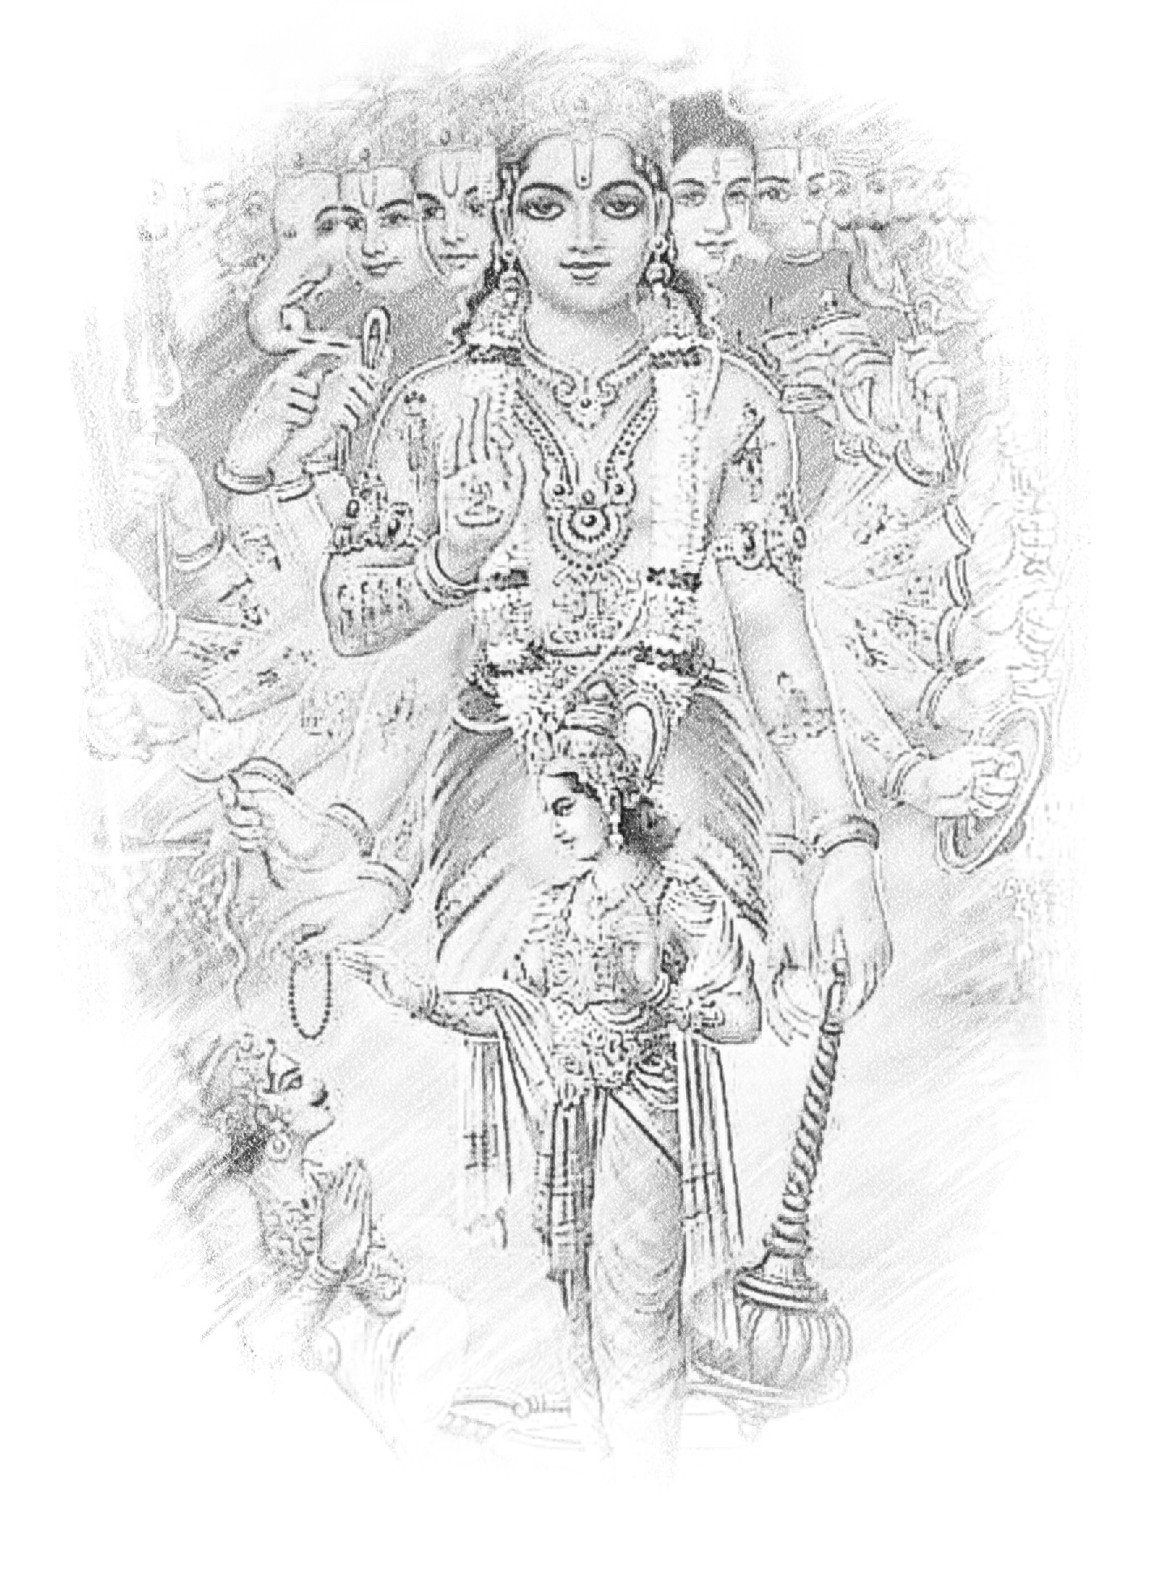
\includegraphics[scale=0.35,keepaspectratio]{CoverImage.jpg}
\end{center}
\chapter*{}
\begin{center}
	
\includegraphics[scale=0.25,keepaspectratio]{eps2}
\end{center}
\pagebreak
\hspace{0pt}
\vfill
\begin{center}
	\sanskrit ललित भाई को समर्पित...
\end{center}
\vfill
\hspace{0pt}
\pagebreak
\chapter*{\sanskrit प्राक्कथन}
\sanskrit

गीता एक अद्भुत पुस्तक है ।  गीता की महत्ता बहुत लम्बे समय से ज्ञात है, इसीलिए गीता का अनुवाद अनेक भाषाओं में हुआ है, परंतु गीता का मूल स्वरुप संस्कृत में है ।  गीता को संस्कृत लिखने से जुडी हुई एक रोचक कथा में यह बताया गया है, कि गीता के लिखने के लिए व्यास ऋषि ने श्री गणेशजी को आमंत्रण दिया ।  लेकिन अपने चंचल स्वभाव के कारणवश गणेशजी ने गीता को लिखने के पहले व्यासजी एक समक्ष यह शर्त रखी व्यासजी को उन्हें लगातार व्यस्त रखना होगा अन्यथा वह ऊबकर चले जायेंगे ।  इसके प्रत्युत्तर में व्यासजी ने भी अपनी एक शर्त रखी कि गणेश कुछ भी समझे बिना न लिखें ।  गणेशजी अपनी तीव्र बुद्धि से व्यासजी का गीतोच्चारण बहुत जल्दी समझकर तुरंत लिख लेते थे, इस पर व्यासजी को श्वांस लेने तक की कठिनाई आने लगी ।  तब  उन्होंने गीता के श्लोको को बीच-बीच में अत्यधिक मुश्किल बनाना आरम्भ कर दिया, जिससे गणेशजी को समझने में थोड़ा समय लगने लगा और व्यासजी को श्वांस लेने का अवकाश मिलने लगा ।  इस प्रकार व्यासजी की इमला और गणेशजी की लिखावट से गीता लिखने का कार्य सम्पूर्ण हुआ ।  लेकिन गीता के श्लोक थोड़े कठिन हो गए ।  उदाहरण स्वरुप पांचवे अध्याय के आठवें श्लोक की दूसरी पंक्ति को पढ़ने की कोशिश कीजिये । 

\begin{quotation}\sanskrit
नैव किंचित्करोमीति युक्तो मन्येत तत्ववित्‌  । 

पश्यञ्शृण्वन्स्पृशञ्जिघ्रन्नश्नन्गच्छन्स्वपन्श्वसन्‌  ॥ ५.८ ॥  
\end{quotation}
जब गीता का अनुवाद अन्य भाषाओँ में हुआ तब ऐसे श्लोकों को संधि-विच्छेद करने के बाद ही लिखा गया, इस कारण अन्य भाषाओं में गीता पड़ना आसान है ।  परन्तु संस्कृत में लिखी गयी गीता आज भी कठिन ही है ।  प्रस्तुत पुस्तक में यह प्रयास किया गया है, देवनागरी भाषा में ही गीता के श्लोकों को संधि-विच्छेद करके लिखा जाए । 

\begin{quotation}\sanskrit
नैव किंचित करोमीति, युक्तो मन्येत तत्व वित्‌  । 

पश्यन् शृण्वन् स्पर्शन् जिघ्रन्न, अस्नन् गच्छन् स्वपन् श्वसन्‌  ॥ ५.८ ॥ 
\end{quotation}
गीता को समझने के लिए कहा जाता है कि कई जन्म लेने पड़ते हैं ।  लेकिन इसका आरम्भ उचित उच्चारण से ही हो तो अच्छा है ।  संधि-विच्छेद के पश्चात आधे से ज्यादा श्लोक देवनागरी पढ़ने वालों को समझ में भी आ सकता है ।  यदि आपको कोई त्रुटि मिले तो कृपया अवश्य बतायें । 
इस पुस्तक के संकलन के लिये मूल श्लोक \textrm{IIT} कानपुर की \textrm{website} से लिये गये हैं ।  \textrm{https://www.gitasupersite.iitk.ac.in}

\begin{quotation}
जय श्री कृष्ण

विश्वजीत अग्रवाल 

\textrm{Vishv.Jeet@gmail.com}

\textrm{January 2021}
\end{quotation}
\AddToShipoutPictureBG*{%
	\AtTextLowerLeft{\makebox[\textwidth][r]{%
			
\includegraphics[scale=0.05,keepaspectratio]{eps4}}}}